% !TEX program = pdflatex
% !TEX options = --shell-escape -synctex=1 -interaction=nonstopmode -file-line-error "%DOC%"
\documentclass[notitlepage]{article}
\usepackage{float}
\usepackage{verbatim}
\usepackage{amsmath}
\usepackage{listings}
\usepackage{bm}
\usepackage{graphicx}
\usepackage{booktabs}
\usepackage{color,xcolor}
\usepackage{enumerate}
\usepackage{minted}

\title{Poisson-FBMP Note}
\date{}

\definecolor{dkgreen}{rgb}{0,0.6,0}
\definecolor{gray}{rgb}{0.5,0.5,0.5}
\definecolor{mauve}{rgb}{0.58,0,0.82}
\lstset{
    language=python,
    basicstyle=\footnotesize,
    numbers=left,
    numberstyle=\tiny\color{gray},
    stepnumber=2,
    numbersep=5pt,
    backgroundcolor=\color{white},
    showspaces=false,
    showstringspaces=false,
    showtabs=false,
    frame=single,
    rulecolor=\color{black},
    tabsize=2,
    captionpos=b,
    breaklines=true,
    breakatwhitespace=false,
    title=\lstname,
    keywordstyle=\color{blue},
    commentstyle=\color{dkgreen},
    stringstyle=\color{mauve},
    escapeinside={\%*}{*)},
    morekeywords={*,...}
}

\begin{document}
\newcommand{\ud}{\mathrm{d}}

\maketitle

\section{P-FBMP with truth prior}

\begin{lstlisting}
tlist = truth['HitPosInWindow'][truth['HitPosInWindow'] < right_wave - 1]
if len(tlist) == 1:
    tlist_edge = np.array([tlist[0] - 0.5, tlist[0] + 0.5])
else:
    tlist_edge = np.concatenate([[tlist[0] - np.diff(tlist)[0] / 2], (tlist[1:] + tlist[:-1]) / 2, [tlist[-1] + np.diff(tlist)[-1] / 2]])
t_auto = (np.arange(left_wave, right_wave) / wff.nshannon)[:, None] - tlist
A = p[2] * np.exp(-1 / 2 * (np.log((t_auto + np.abs(t_auto)) / p[0] / 2) / p[1]) ** 2)
t0_t = t0_truth[i]['T0']
mu_t = len(truth)
factor = np.sqrt(np.diag(np.matmul(A.T, A)))
A = np.matmul(A, np.diag(1. / np.sqrt(np.diag(np.matmul(A.T, A)))))
la = mu_t * np.array([integrate.quad(lambda t : wff.convolve_exp_norm(t - t0_t, Tau, Sigma), tlist_edge[i], tlist_edge[i+1])[0] for i in range(len(tlist))]) + 1e-8
xmmse, xmmse_star, psy_star, nu_star, nu_star_bk, T_star, d_tot_i, d_max_i, num_i = wff.fbmpr_fxn_reduced(wave_r, A, la, spe_pre[cid]['std'] ** 2, (gsigma * factor / gmu) ** 2, factor, len(la), stop=5, truth=truth, i=i, left=left_wave, right=right_wave, tlist=tlist, gmu=gmu, para=p)
c_star = np.zeros_like(xmmse_star).astype(int)
for k in range(len(T_star)):
    t, c = np.unique(T_star[k][xmmse_star[k][T_star[k]] > 0], return_counts=True)
    c_star[k, t] = c
mu = np.average(c_star.sum(axis=1), weights=psy_star)
t0 = t0_t
\end{lstlisting}

Use true \texttt{HitPosInWindow} as \texttt{tlist}, true \texttt{T0} as \texttt{t0\_t}, length of \texttt{HitPosInWindow} as \texttt{mu\_t}. \texttt{la} is vector of integral in each time bins. 

\begin{figure}
    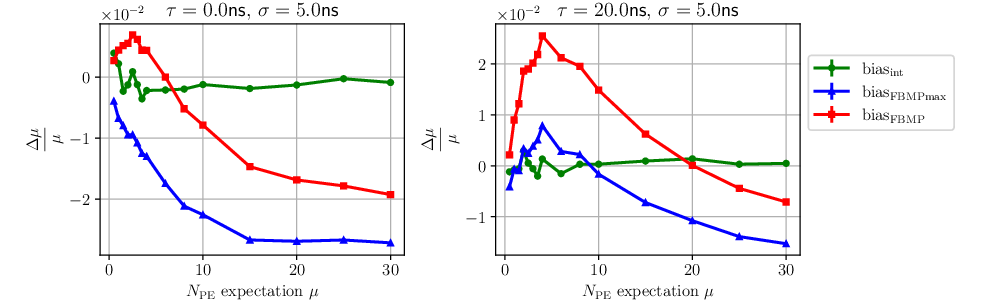
\includegraphics[width=\textwidth]{vs-biasmu.png}
\end{figure}

\end{document}